Original image was loaded from the ENVI format with the interleave format BIL. The image was saved with the interleave format BIP. The Python script is shown in Code \ref{code:save-bip}.

Function \texttt{load\_spectral\_image} in \ref{code:save-bip} is defined in Code \ref{code:load-envi}.

The header file of the BIP image is shown in Code \ref{code:header-bip}. There are two changes from original one: description and interleave method.

The preview by FreeLook is shown in Figure \ref{fig:bip-preview}.

\begin{figure}[H]
  \centering
  \caption{Preview of BIP image by FreeLook}
  \label{fig:bip-preview}
  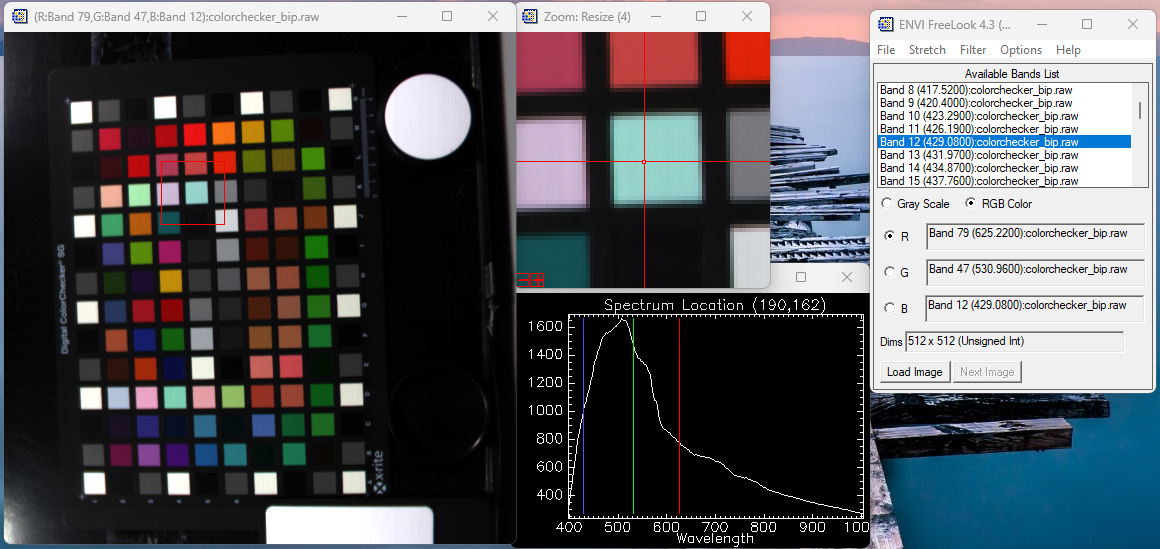
\includegraphics[width=0.5\textwidth]{./fig-task4/bip_preview.png}
\end{figure}

\begin{lstlisting}[caption=Header file of BIP, label={code:header-bip}]
ENVI
description = {Data transformed to BIP}
samples = 512
lines = 512
bands = 204
header offset = 0
file type = ENVI
data type = 12
interleave = BIP
sensor type = SPECIM IQ
byte order = 0
default bands = {70,53,19}
latitude = 0.00000000
longitude = 0.00000000
acquisition date = 29-09-2020
errors = none
binning = {1,1}
tint = 121
fps = 8.26446
wavelength = {
    397.32,
    400.20,
    403.09,
    405.97,
    408.85,
    ...
}
\end{lstlisting}
